 \documentclass[10pt,a4paper,headinclude=true,twoside]{report}
\usepackage[latin1]{inputenc}
\usepackage[a4paper]{geometry}
\usepackage{a4wide}
\usepackage{amsmath}
\usepackage{amsfonts}
\usepackage{amssymb}
\usepackage{graphicx}
\usepackage{hyperref}
\usepackage{pdflscape} % dlia landscape orientation 
\hypersetup{colorlinks,citecolor=black,filecolor=black,linkcolor=black,urlcolor=black}
\usepackage{float}
\usepackage{setspace}
\usepackage{titlesec}
\titleformat{\chapter}
  {\Large\bfseries} % format
  {}                % label
  {0pt}             % sep
  {\huge}           % before-code

\usepackage{fancyhdr}
\pagestyle{fancy}

\fancyhead[LE,RO]{\slshape  \rightmark} %should be used with "twoside" in documentcalss. Delat headeri kak v knigah: vneshnije storoni sovpadajut drug s drugom. 
\fancyhead[LO,RE]{\slshape  \leftmark}
\fancyfoot[C]{\thepage}

%\lhead{Edgar Ivanov}
%\rhead{Industrial Year Report}
%\cfoot{\thepage}

%\pagestyle{myheadings}

%\usepackage{biblatex}

\renewcommand{\familydefault}{\sfdefault}

\begin{document}
\onehalfspacing
\title{Industrial Year Report \\ Aberystwyth University Information Services}
\author{Edgar Ivanov\\ edi@aber.ac.uk \\ Department of Computer Science, Aberystwyth University}
\date{\today}

\maketitle

\newpage
\thispagestyle{empty}
\mbox{}

\tableofcontents

\chapter{Organization}
My industrial year placement takes place at Aberystwyth University, in the Information Services department (further will refer as "IS"). Aberystwyth University is an institution of higher education, which provides undergraduate and postgraduate education. AU is located in Aberystwyth town, on the west coast of Wales, with average population of 15 thousand people. The University was founded in 1872 as University College Wales and has changed its name since then a few times \cite{History}.
The University has 17 academic departments and 27 service departments \cite{Departments} \cite{Departments2}. Most of the teaching departments are located on Penglais campus, as well as on Llanbadarn campus within 15 min. walk from Penglais and in the Old College, where Welsh History department and managerial staff are located. There is a big research department called IBERS as well (Institute of Biological, Environmental and Rural Sciences), it used to be an independent organization but then joined the AU.

\section{Information Services}
IS department provides the University with Library, IT, Management Information and Media Services. There are three main sub-departments within IS: Business Information Systems, ICT \& Customer Support and Library Services (figure~\ref{fig:i-s-hierarchy-tree-march-2012}), each of them is then broken down in to smaller groups and teams that have different roles and responsibilities.

\begin{figure}[H]
\centering
\centerline{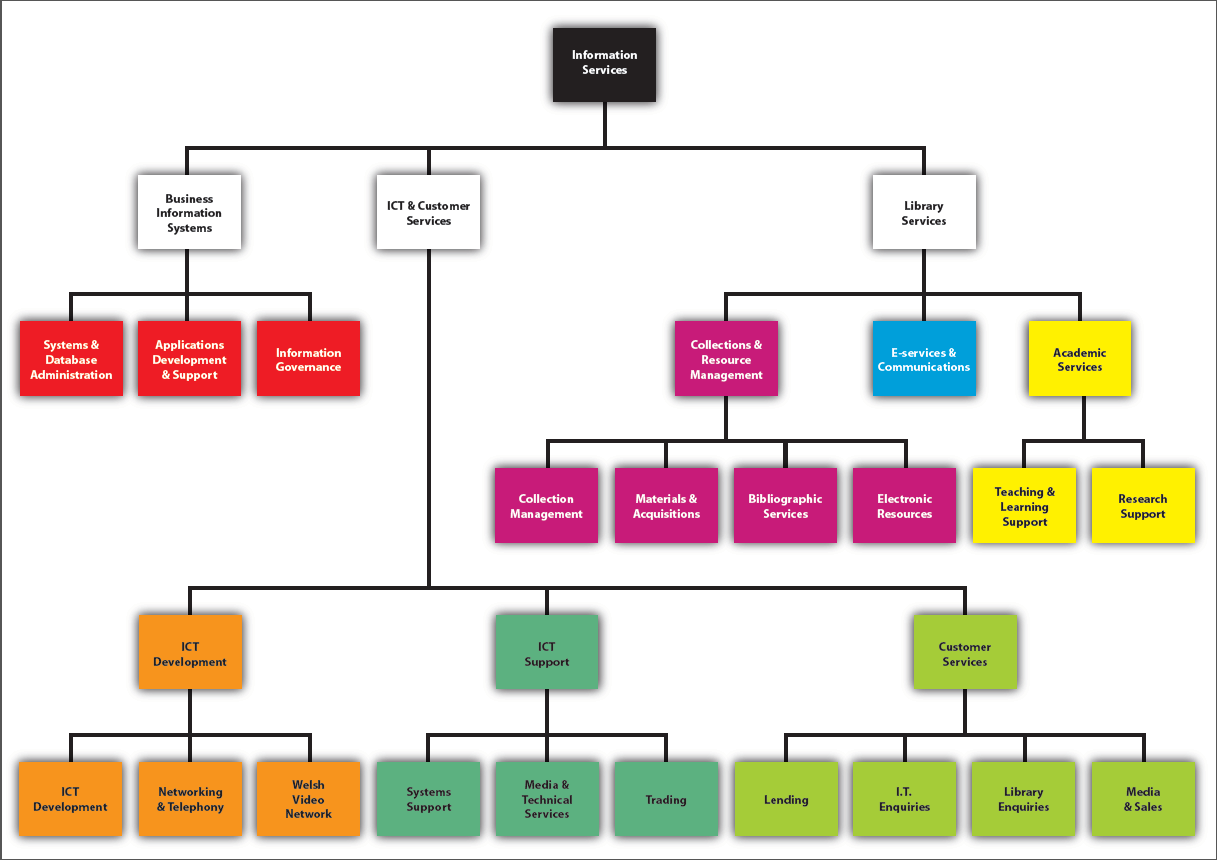
\includegraphics[scale=0.55]{./i-s-hierarchy-tree-march-2012}}
\caption{IS hierarchy tree \cite{ISHierarchyTree}}
\label{fig:i-s-hierarchy-tree-march-2012}
\end{figure}

IS department is located in Hugh Owen building and takes over 40 \% of the E floor.  Figure~\ref{fig:isfloorplan}  represents  IS staff location plan. Most of the IS department employees are based in the open plan office, with the team leaders located in the offices at the edges. My workplace was in the Computer Workshop, which is separated from the main office.

\begin{figure}[H]
\centering
\centerline{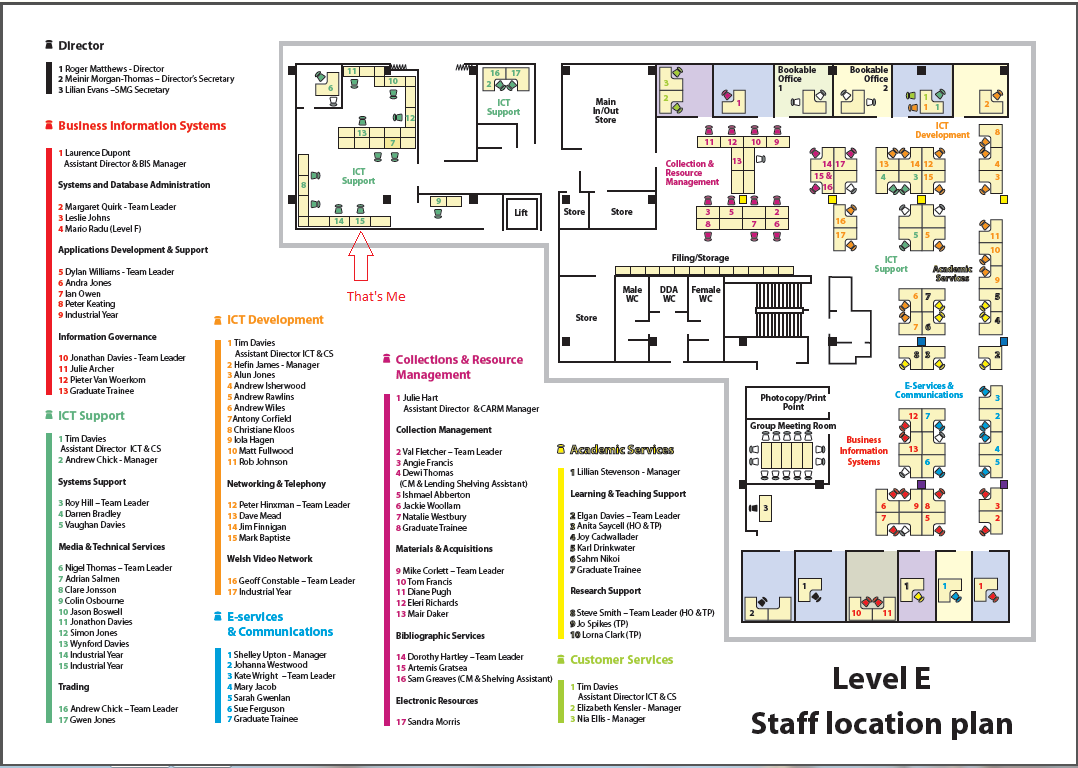
\includegraphics[scale=0.55]{./isfloorplan}}
\caption{IS staff location plan \cite{ISFloor}}
\label{fig:isfloorplan}
\end{figure}

\section{ICT Support}
This group is responsible for ICT equipment provision and support. In the following sections I will describe sub-teams in detail.
\subsection{Media \& Technical Services (My Team)}
The team that I am based in falls under IS $>$ ICT \& Customer Services $>$ ICT Support and is called "Media \& Technical Services", people in IS usually refer to it as to "Workshop". It is defined as a group responsible for the software and hardware upgrades and repairs a wide variety of ICT equipment types. It also provides multimedia services and supports ICT equipment within teaching spaces. All computer relevant hardware repairs are being done here, which includes internal repairs (equipment owned by the University) as well as repairs for external customers (staff, students, members of publicity). The members of this group provide the lecturers who experience the difficulties with the ICT equipment in the classrooms with the technical support. 

Computer workshop acts as a second line of contact for the customers and deals with complicated issues that could not be resolved within the reasonable time frame by the help desk staff. IT Enquiries group deals with all incoming phone calls and emails. Usually over 90\% of all enquiries are resolved at this stage. If there is something that requires physical technician presence or problem cannot be resolved remotely or at the help desk, then a staff member opens a new call in our job management system and assigns a job to the appropriate team. That is how workshop team gets most of the jobs. Then the jobs are distributed to the team members by our team leader or technicians pick up the jobs themselves. The jobs that we receive vary greatly from each other, in most cases it is something that requires advanced knowledge in IT, e.g. laptop fix after spillage, the printer that isn't working, slow computer performance, virus removal, delivery and configuration of the new IT equipment, malfunctioning IT equipment diagnostics. Sometimes we get unusual jobs and we don't have appropriate equipment or an appropriate qualification to deal with them. I remember a case when the customer requested to measure the signal strength of the antenna, he was then referred to an external company.

There are eight people working in the computer workshop on a permanent basis, one graduate trainee who joined us in January for a year and two industrial year placement students like me, who work on a rotating basis and change every year. Most of the full-timers have relevant education, are A+ certified\cite{A+} and have previous experience in supporting IT equipment. Computer workshop is also certified service provider for Toshiba and Apple Inc. and performs warranty repairs for computers, out of warranty repairs for any other brand computers can be performed here for a charge. 

I would describe Workshop as a relaxed work environment which allows all of us to talk freely to each other whilst remaining focused on our duties and completing the jobs we are assigned to. During the first month I was trained by previous industrial year student employees (they left at the end of the first month of my placement to continue their studies), they showed me some systems that we used, helped to deal with my first jobs and provided me with advice. After them leaving I could seek advice from anybody in the workshop, people were very friendly and helpful, they would explain all I need to do, although not mentioning or skipping some details and I had to find them out myself.
\subsection{Systems Support}
This group is responsible for all the aspects of public service computers, including software licensing, purchasing, management and implementation for IS and many departmental products. It makes backups for most of the University's systems and maintains two main server rooms, one in Penglais and one in Gogerddan. It also provides second/third line software support for the help-desk/workshop.\cite{InternalTeamdescription}
\subsection{Trading}
It offers a wide range of computers, laptops, media equipment and peripherals for sale to University departments, individuals and external customers. Prices are generally competitive and are often at specially negotiated educational terms and/or with extended warranties for the members of the University.\cite{InternalTeamdescription}
\section{ICT Development}
Designs and implements systems and services for IS, other University departments and external bodies. It also develops, implements, trains and supports IS users on bespoke software and ensures existing systems are efficient and cost effective. This includes Network and Telephone service design promoting standardization and centralization and managing improvements and information security incidents.\cite{InternalTeamdescription}
\section{Customer Services}
Provides Lending, ICT enquiries, Media \& Sales and Library Enquiry services for staff, students and visitors. Monitors the responsiveness and effectiveness of front-line services, ensures services best meet users' needs and promotes awareness of IS enquiry and front-line services. It also manages services and staffing for Fresher's Weekends and students' induction programmes.\cite{InternalTeamdescription}
\subsection{I.T Enquiries}
The first point of contact for face-to-face and online IT enquiries for all IS users. Troubleshoots any problems users experience with accessing or using IS services and resolves them or refers them as appropriate. It also supports the public printing service, facilitates access to IS services such as email accounts, Aber cards, computing network, and printing and represents users within IS e.g. presenting user feedback at the meetings or user testing new services. \cite{InternalTeamdescription}

I spend a few hours a week within this team. I am usually working on the help desk where students and staff come with various questions.

\section{BIS and Library Services}
There also are two other sub-departments called "Business Information Systems" and "Library Services". People in BIS are  responsible for the development and support of the systems and processes required to maintain Admissions, Student Records, Finance, HR, Payroll and other associated business functions of the University. Library Services department looks after all the education materials: books, journals, articles as well as after education software systems like "AberLearn Blackboard".\cite{InternalTeamdescription}

\section{Summary}
I think it is a very professional organization, with each team responsible for provision and maintenance of the specific service; they control their section entirely and no one else is entitled to take over their work. At the same time teams within the IS department collaborate and work together on matters that affect more than one team. There is also a logical hierarchy of management staff: director -$>$ manager -$>$ team leader; they ensure that staff feedback is taken into account at the highest level. People in IS work collaboratively to provide the best service for the end user and ensure the services continuity. I felt working in a highly professional organization where everybody knew their place and were experts in their field of knowledge.

\chapter{Customers}
I decided to devote the whole chapter to the IS department customers. To get a full picture it is essential for the reader to understand who we provide support to.

The majority of the IS customers are University staff and students of different age, although we do occasionally get requests from the external bodies or private customers. All the customers have different level of knowledge in IT. Quite often I found myself explaining people how to use shortcuts on keyboard efficiently and other basics. The difference in the knowledge has also required me to treat them differently, because quite a few customers would not understand the terminology I used.  

Computer workshop provides similar service for staff, students and external customers in terms of ICT equipment repairs. If there is a lot of work, priority is usually given to the equipment owned by the University.

When a customer drops off his laptop in the workshop or when I collect a broken computer, people want to know how quickly their fault will be fixed and try to be pushy about the time frame in which a fault should be resolved. At the beginning of my placement that was a bit stressful because I tried to satisfy everyone at once promising that their fault would be fixed within the 3 days time and then rushing to do the job fast to keep the promise. Impossibility to keep the promise due to overloaded schedule was making my customers unhappy and me frustrated, as well. It had lasted for a while until I have realized the usefulness of the approach and started concentrating properly on one fault instead of trying to fix ten of them at the same time. I discussed the issue with my team leader and have also asked my colleagues to share their experience with me. I am now trying to give a blurred time frame so that the customers would not expect to see their equipment back at least for a few days or a week. 

As you can see, the diversity of customers is wide, so is the variety of issues we deal with.

\chapter{Technical environment}
When I've just started my placement I was amazed by the amount of different software used in IS and how the information was spread across the systems. At the beginning I was introduced to the Interzone, Sunrise, Astra, Recall, SharePoint, Aber FAQs, Outlook, Voyager. All of these use to store different kind of information and help people with their day-to-day duties. In this section I will go through technical environment and describe what software and tools I use when doing my job.
  
\section{My Work Environment (Computer Workshop)}
Computer Workshop is an open plan office as shown on figure ~\ref{fig:isfloorplan} that consists of our workbenches and team leaders office in the corner. At the beginning of my placement I was given a place at the workbench and a computer capable of doing simple office tasks. There are tools in the computer workshop that you would expect to see in any more or less advanced household: this includes screwdrivers, pliers, soldiering kit, heat gun, drill, hex keys, different types of wrenches. There also are some specific tools that are used only for computer hardware diagnostic and repair: power adapters and PSUs (power supply units), PATA and SATA computer data cables, HDD (Hard Disk Drive) cloners, magnifying glass to detect liquid damaged components, all of our workplaces are grounded and have antistatic wrist straps and anti-static mats to prevent electrostatic discharge when working with sensitive computer components, network cable testers, multimeter. We also have a store room to keep new computer components such as new HDDs, cables, monitors, laptop screens, PSUs in case we need any of them during a repair.    

Computer Workshop Technical Environment is very unusual in comparison to the rest of the IS. We not only deal with software related issues here, but the hardware as well: soldiering, computer part replacement, cleaning the equipment after spillages, equipment shifting, hardware diagnostics, all unusual jobs come here.

When a term starts we tend to get quite a lot of laptops that fail to boot in to the OS. Usually it is caused by damaged HDD, having broken sectors that cannot be read. In such cases Diskology Disk Jockey PRO hard disk cloner\cite{DiskCloner} becomes extremely useful since it can skip broken sectors, filling them with zeros on the destination drive and making it possible to copy the data from the source drive. Some files may become damaged, but this is still better than having no data at all. We also tend to get requests to restore lost data from USB pen drives and SD flash cards - then we use R-Studio, a program which performs the scan of the whole drive and then displays all the data that is available for recovery. 

Symantec Ghost is a disk cloning program, capable of making one-to-one copy of any storage media (HDD, SD Card, USB Pendrive). Symantec Ghost is used heavily during MS Windows OS deployment on public computers. When reference Windows OS installation is complete and all the necessary programs are installed, the whole HDD is being captured in to the file, then computers join multicast session and the image that has been captured before is applied to all of the machines. It is a very effective technique, because there is no need to spend hours with each computer installing Windows OS with all the corresponding applications. Usually, we deploy image to the 50-100 computers in one go, the size of the image is around 50 GB(that is MS Windows 7 OS, with almost 200 applications required for the education use) and that is when Symantec Ghost multicast ability becomes useful, data is sent from one source to all the computers simultaneously in a single transmission and does not overload our network. We can have 50-100 computers ready for use within 5-12 hours using this technique, which couldn't be achieved without it.

To remove viruses from the computers we use Sophos Endpoint Antivirus and Microsoft Security Essentials, both of these applications proved to be effective.
 
\section{Interzone}
Interzone is a front end web interface for the database that is used to manage records of the network equipment in Aberystwyth University. It contains comprehensive data about the device including information about the owner. All the equipment connected to the University network has its MAC (media access control) address registered in our database, otherwise our DHCP server will not assign IP address to the device and without the IP address a device will not be able to use our network facilities.

On the main page it is possible to specify search criteria and look for devices that match the request. Some of the search criteria are: IP address, MAC address, Owner's login, computer name. On the figure ~\ref{fig:main_interzone_page} you can see the main Interzone page.

\begin{figure}[H]
\centering
\centerline{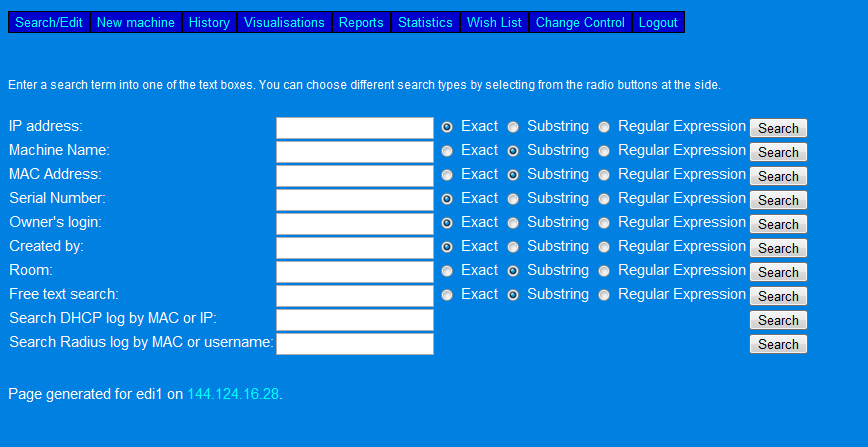
\includegraphics[scale=0.5]{./main_interzone_page}}
\caption{Main Interzone Page}
\label{fig:main_interzone_page}
\end{figure}

On the figure ~\ref{fig:machine_record} Interzone record of my computer.

\begin{figure}[H]
\centering
\centerline{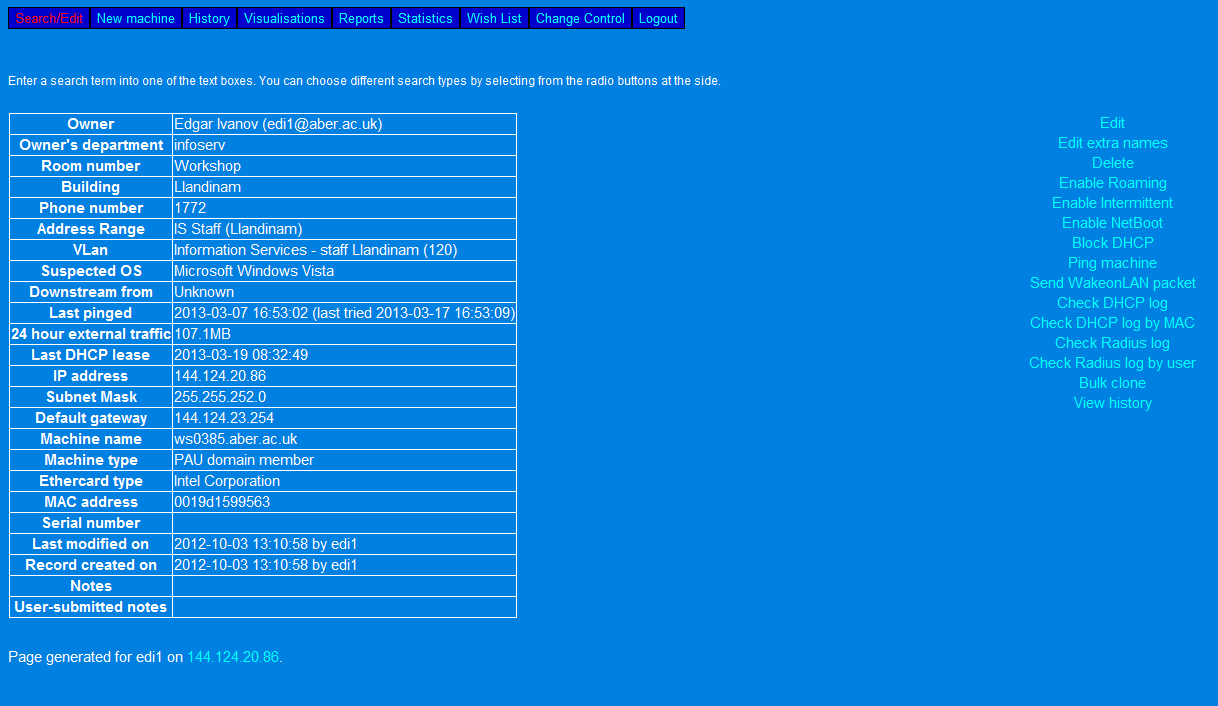
\includegraphics[scale=0.5]{./machine_record}}
\caption{Machine record}
\label{fig:machine_record}
\end{figure}

It contains various information about the owner, owners department, telephone number, VLAN, IP and MAC addresses, the type of the device (PC, laptop, switch). You can find some other useful information there too.

\begin{figure}[H]
\centering
\centerline{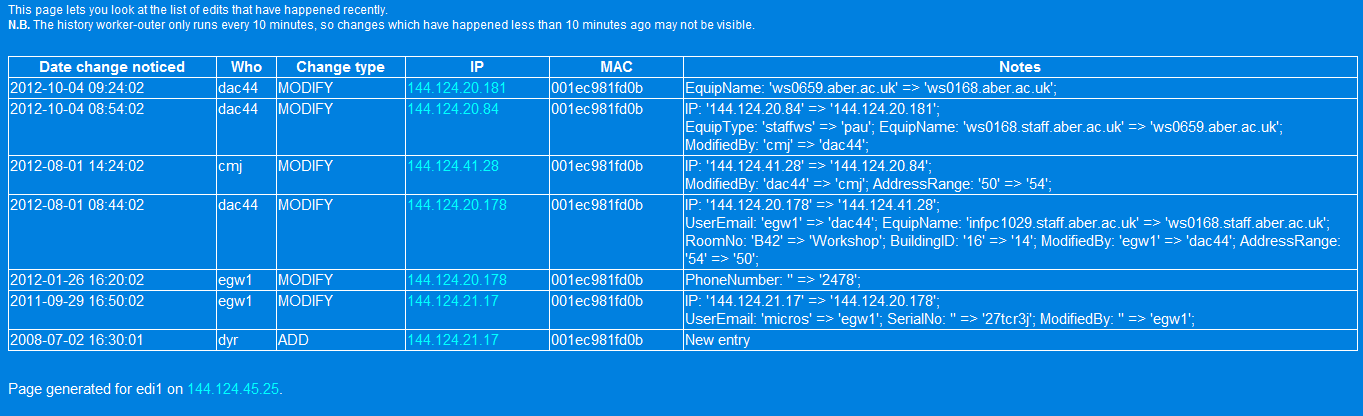
\includegraphics[scale=0.5]{./modification_history}}
\caption{Modification History}
\label{fig:modification_history}
\end{figure}

The information gathered from Interzone can be very useful when troubleshooting computer connection issues. It is possible to check DHCP log to see if the computer gets IP address, look at the RADIUS logs that contain information about the user being successfully or unsuccessfully authenticated in our system. Figure ~\ref{fig:interzone_radius} shows RADIUS log for my mobile phone, it is possible to see that my phone was unable connect to the network due to the authentication problem at some point (I have intentionally changed the password to the wrong one). When working on the help desk and troubleshooting devices which were not connecting to the network properly, Interzone logs let me know what was going wrong so that I could choose an appropriate solution. 

\begin{figure}[H]
\centering
\centerline{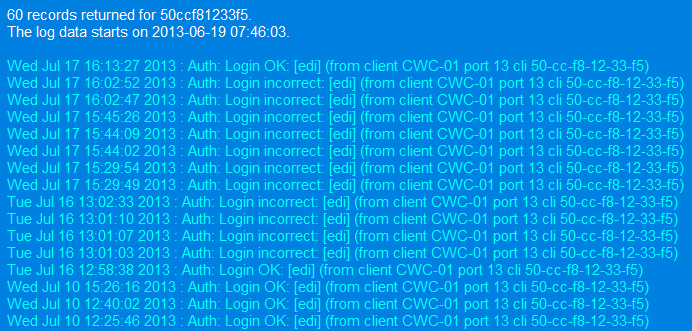
\includegraphics[scale=0.5]{./interzone_radius}}
\caption{RADIUS log}
\label{fig:interzone_radius}
\end{figure}

Interesting reports are generated from the information contained in the database, one of them is on the figure ~\ref{fig:interzone_statistics}, showing the total amount of records in the database (that is pretty much how many physical devices are using University network).

\begin{figure}[H]
\centering
\centerline{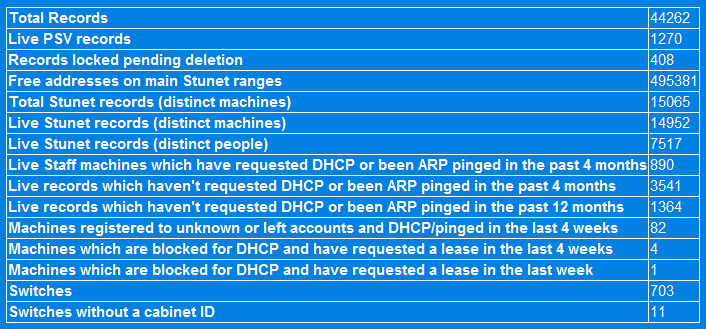
\includegraphics[scale=0.5]{./interzone_statistics}}
\caption{Interzone Statistics}
\label{fig:interzone_statistics}
\end{figure}

\section{Sunrise}
Sunrise is another front end web interface for the database that I use to keep track on current and past calls. This job management system is used to create new "jobs", allocate them to the technician or to the team, add the comments about the job, send emails to the user with updates etc. Almost all the jobs are coming to the workshop from the help desk, when first line fix is not possible the request is created with necessary information filled in. After the job is assigned to my team our team leader redirects them to the technicians or technicians pick up a job themselves, which happens far more often. On the figure ~\ref{fig:sunrise_main} there is main Sunrise page, with all ongoing jobs assigned to me. There are boxes where you can specify the search criteria and look for the specific job.

\begin{figure}[H]
\centering
\centerline{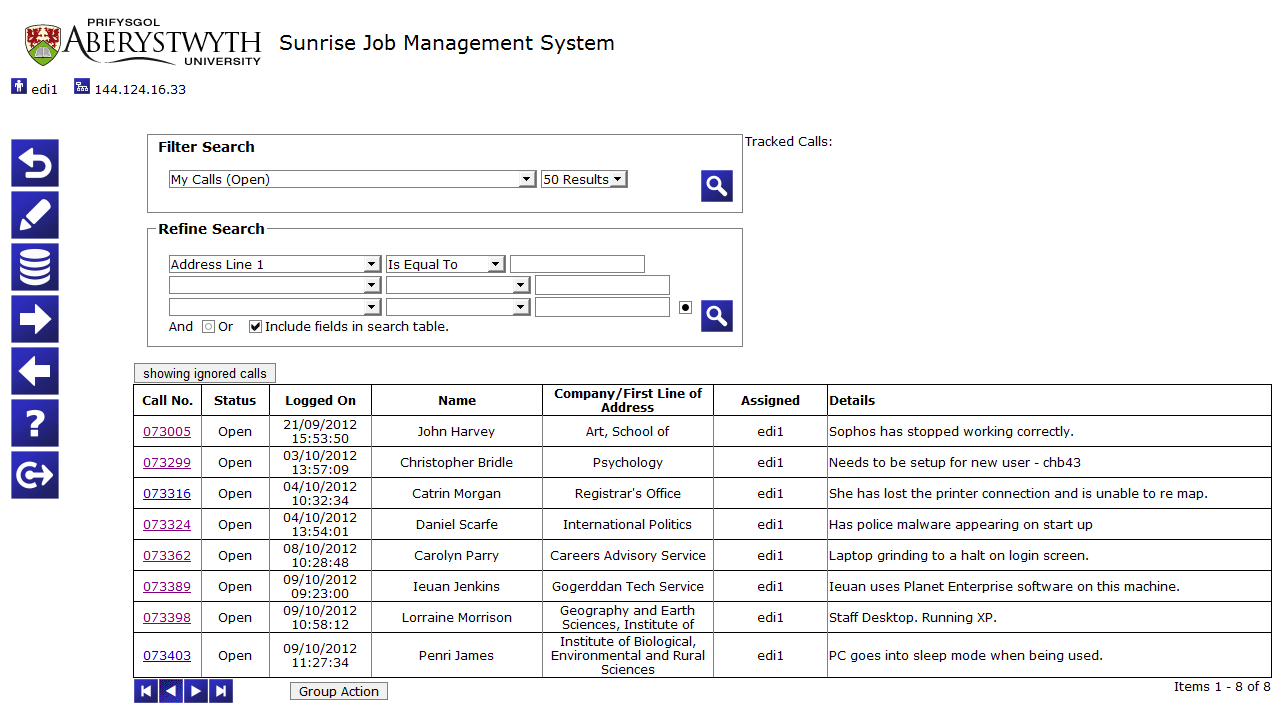
\includegraphics[scale=0.5]{./sunrise_main}}
\caption{Sunrise Main Page}
\label{fig:sunrise_main}
\end{figure}

Figure ~\ref{fig:sunrise_search} shows all the jobs that contain my email address "edi1" in them.

\begin{figure}[H]
\centering
\centerline{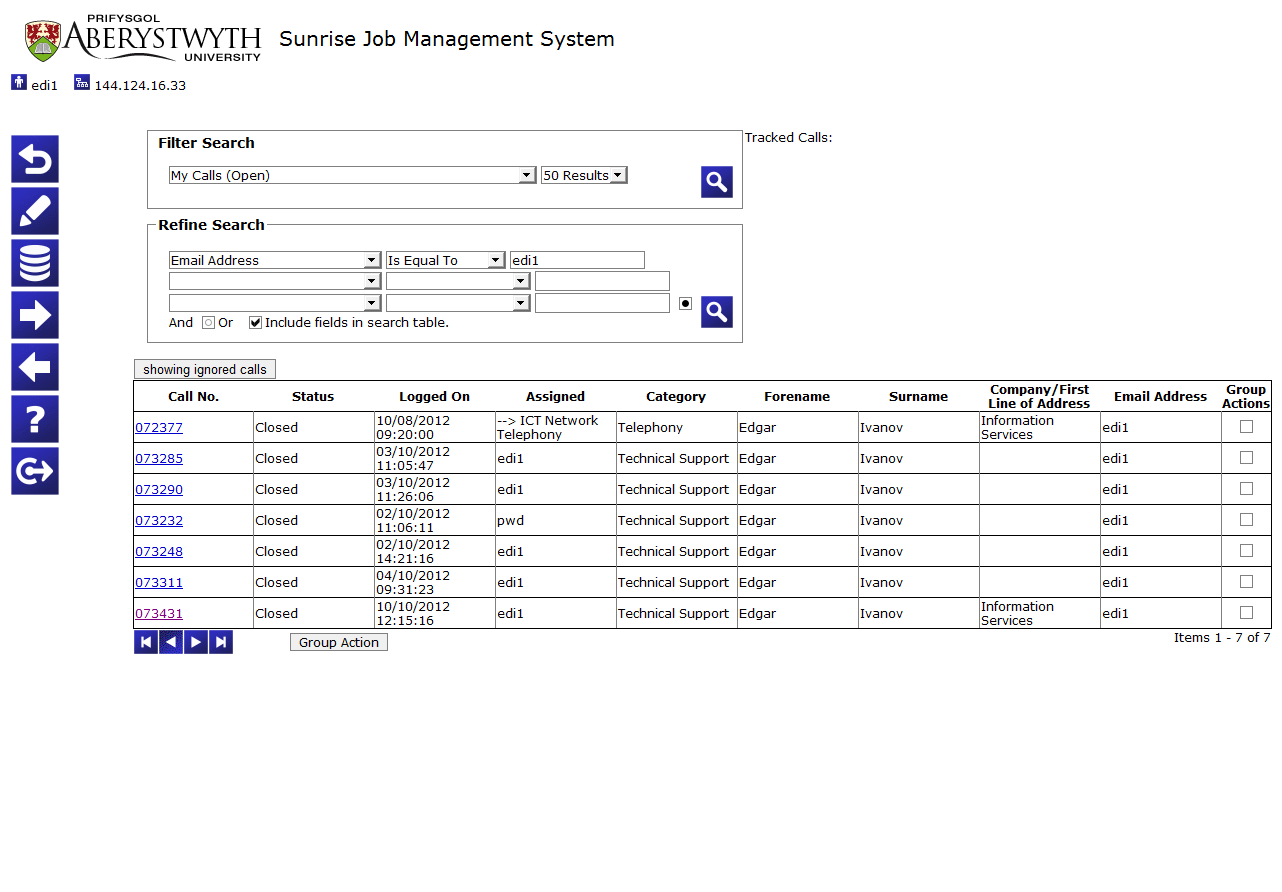
\includegraphics[scale=0.4]{./sunrise_search}}
\caption{Sunrise Search}
\label{fig:sunrise_search}
\end{figure}

Figure ~\ref{fig:sunrise_job} represents a job to be completed. Each job has a unique Call Number, which is 075028 in this case, it also has the email address of the person the job was opened for, his phone number, address, equipment serial number, equipment description (laptop, desktop PC, projector, printer) and any comments where a fault or an issue is described. On the right hand side there is job history pane, each action that technician performs must be added to the history, it helps others to see what was done so far or is planned to be done. Some equipment comes to the workshop more than once and it may be handy for the technician to see what was done in the past.

\begin{figure}[H]
\centering
\centerline{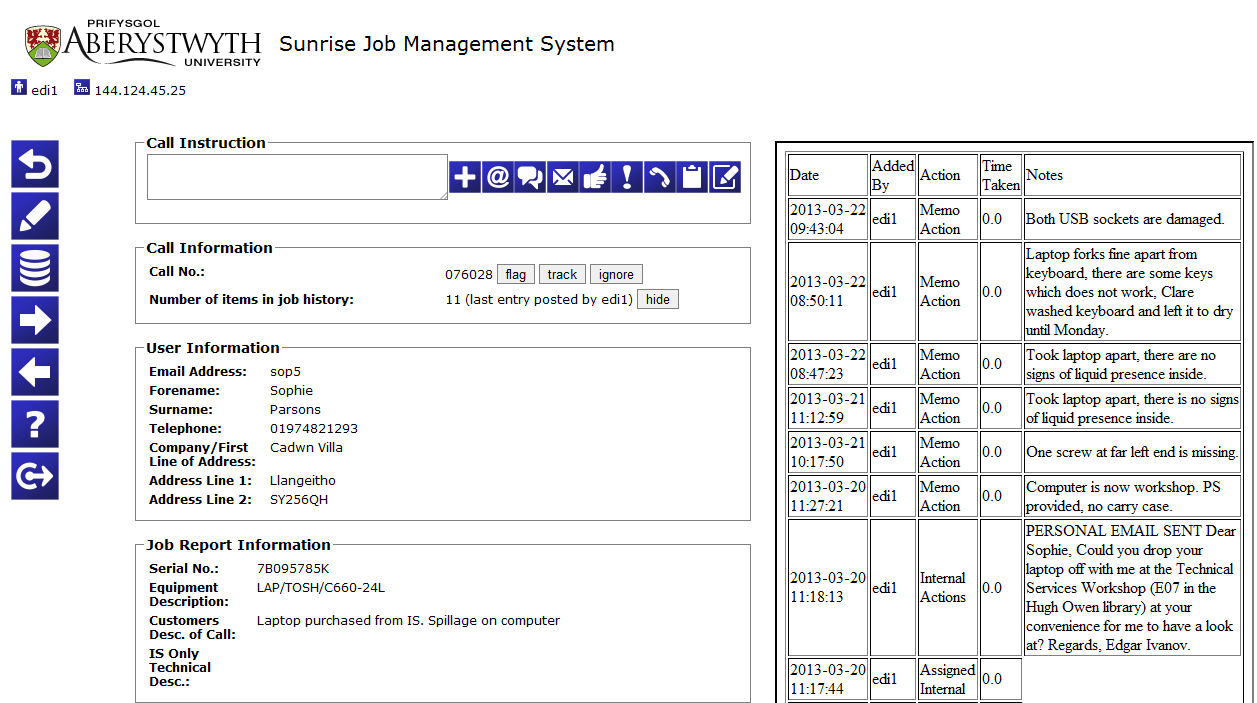
\includegraphics[scale=0.5]{./sunrise_job}}
\caption{Sunrise Job Record}
\label{fig:sunrise_job}
\end{figure}

\section{REG}
Whenever somebody becomes a part of the University (students, staff, visiting staff) a user account is created for them. Username is allocated by the system and usually consists from three letters and some digits if required, for example mine is "edi1". Users then can use them to access their emails, e-journals, manage records about themselves and login to all the systems in the University (if they have access to them). We have web interface called REG to help us manage the accounts. I was mainly using it for unlocking the user accounts while working on the help desk, issuing new passwords, verifying identity of the people at the desk. One of the options I had was to make temporary password for any user, so that I could use their login if required. It was quite useful when I needed to migrate user profile folder on Windows OS and user was away or it was not feasible for them to come in the workshop. In such cases I would create temporary password, login on the computer using their credentials (that is when Windows creates an actual folder for the user together with the other corresponding registry entries), log off and revert the password back. I could then copy all the files from the one machine to the another and be sure that everything will work after the machine is delivered and user logs in.
\section{SNMPc network manager}
Aberystwyth University is a large organization, having thousands of devices connected to its network. To be able to provide reliable service to the end users we need to ensure that our network functions properly and issues are fixed as soon as possible. Network equipment such as: computers, printers, IP cameras, SALTO locks, wireless access points, VoIP phones all relay on ability to communicate (send/receive data), so it is crucial to ensure that there is working network connection at all times.  To monitor all our switches, routers, servers, workstations and printers IS uses a program called SNMPc, developed by Castle Rock Computing. SNMPc is a Distributed Network Manager \cite{SNMPc} that uses SNMP protocol(Simple Network Management Protocol) to communicate and monitor the devices. SNMPc makes it easier to look after the whole network and network devices by identifying unresponsive equipment or network path with the issues and highlighting problematic devices on the network map. 

Figure ~\ref{fig:SNMPc_main} shows a map of our network in SNMPc program. Each icon represents a building, hall of residence or a separate piece of the network, the solid lines between the icons represent fibre optics and thinner lines represent gigabit Ethernet links. Green or purple icon shows that all nodes within are contactable. If an icon turns red it indicates that at least one node in this sub map is not contactable any more \cite{SNPMcSharePoint}. It is enough to give a quick look at the map to identify if there are any issues on the network. I didn't use this application much since there are other people responsible for keeping our network up and running, but I found it quite interesting and useful to look at it from time to time. I can see and explore our network in graphical view, it gives me some understanding of how corporate network should be configured and I will definitely use the knowledge in future.

\begin{figure}[H]
\centering
\centerline{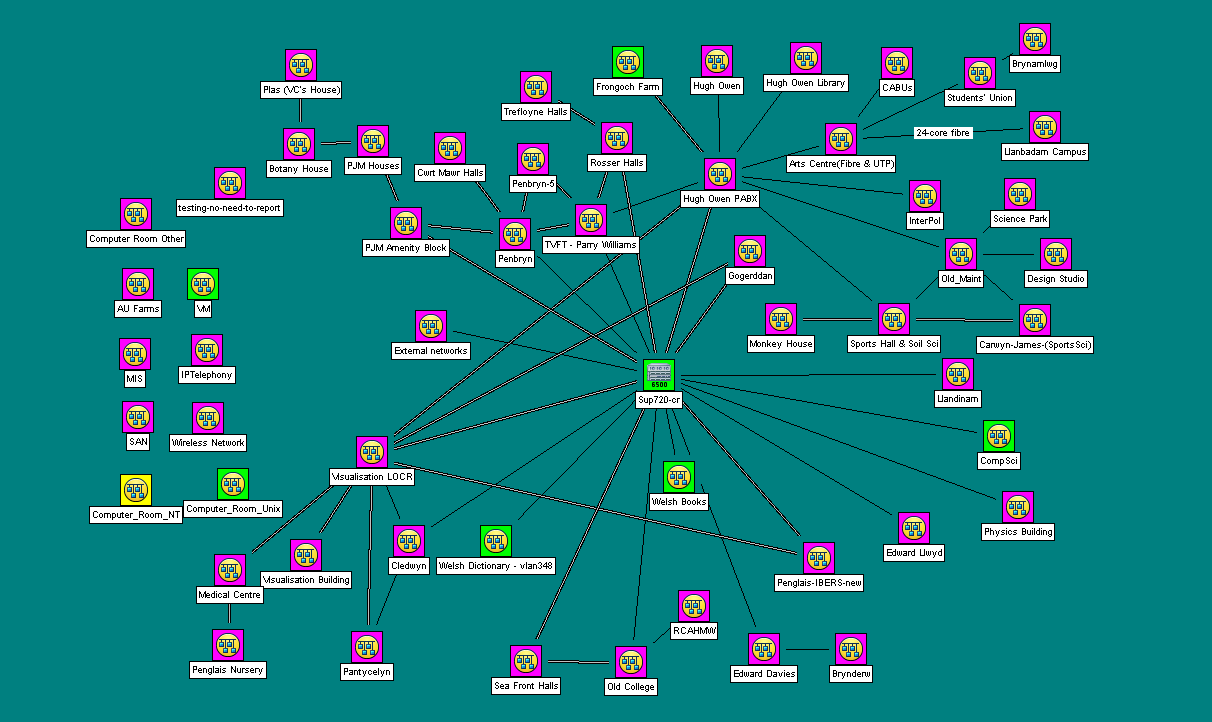
\includegraphics[scale=0.5]{./SNMPc_main}}
\caption{University network map in SNMPc application}
\label{fig:SNMPc_main}
\end{figure}

\section{PCounter}
PCounter is application that allows to  manage user print profiles. It allows to see print balance for everybody in the University, it is possible to increase or decrease balance on the account, see print history and produce reports. I used it mainly for adding money to the user accounts when print credit machine was broken and users were coming to the desk to top up their balance.

\section{VoIP Phones}
Right in the middle of my placement IS has finished a big project of VoIP phones roll-out in the whole University \cite{VoIP}. VoIP stands for "Voice over Internet Protocol" which means that voice data is carried over the Internet instead of public switched telephone network \cite{VoIP2}. There are numerous advantages of using VoIP phones over the usual ones, VoIP phones can display the callers name acquired from the corporate directory, it has extension mobility which means that a user can log in to any phone with their credentials, they can deliver a voice mail directly to the users email inbox. Most of the phones get the power from the Ethernet cable (Power over Ethernet), so there is no need to have a power outlet nearby. When I was on calls in different departments and needed to make a phone call to somebody in the IS I was using a feature in the phone that allows to find the user phone number by their name. There is also a possibility to install "softphone" software on the computer which allows to use computer and internet connection to make telephone calls instead of the usual handset and telephone line \cite{VoIP3}. It is very useful when the staff works from the home and have to receive phone calls from the colleagues, they are reachable on the same extension number as if they would be in the office. It is also possible to manage all phone aspects remotely with Cisco Unified Communications Manager. With VoIP phones there is no need in dedicated Telephone Exchange equipment, all it needs is a software running on the server that handles all requests from the phones and manages the whole phone infrastructure.
 
\section{M drive}
The "M" drive is known by the staff and the students as a network file store, where they can keep any kind of information, the same as on USB pen drive and it is accessible from any computer that has an access to the Internet. The size of the file store is limited to 2 GB per user.  It is a very convenient since the information is stored on University servers and there is no need to carry any physical media. IS makes regular backups of all "M" drives, so if the user deleted something accidentally it would be possible to recover the file from the backup. When users log in onto the computers in the University computer rooms, filestore is automatically mapped on the computer as "M" drive \cite{MDrive}.

\section{Computers}
Here at Aberystwyth University we have hundreds of computers used across campuses by both the staff and the students. While the computers used by the staff members may vary greatly in configuration, all public computers used by the students have the same hardware and software configuration across the campuses.
\subsection{PSVs}
PSVs (Public Service) are computers that can be used by anybody who have University's user account. IS manages around 500 public computers across the campuses \cite{PSVs2}. We have two different versions of Optiplex 7010 computers. One model with higher specifications for teaching stations and USFF model for the student use. 

This summer we deployed new USFF Dell Optiplex 7010 \cite{PSVs} computers, since old ones were almost seven years old and didn't match current student and staff needs. New computers are more powerful, equipped with Intel i3 processors, 4GB of RAM and 320 GB HDDs. All PSVs run MS Windows 7 OS and are "PSV" domain members which makes their management more easy, there are more than 200 applications installed for the academic use. A few computer rooms (from 25 to 100 PCs in one room) are available for teaching purposes and for general use.
\begin{figure}[H]
\centering
\centerline{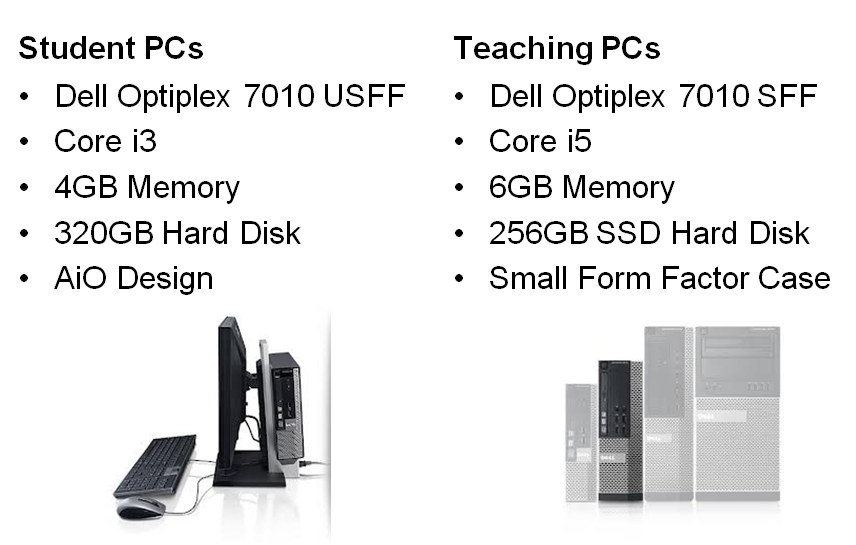
\includegraphics[scale=0.5]{./PSVs}}
\caption{Public workstation PCs \cite{PSVs}}
\label{fig:PSVs}
\end{figure}
\subsection{Staff Computers}
In Aberystwyth University departments are responsible for buying computers for their staff members, the money for that purpose are allocated from the department's budget. All of the purchases go through IS. After IS are informed of the computer choice, it goes through "build" process - all the necessary software is installed and PC is joined to the domain. 

I am dealing with a wide variety of the staff computers, most of them are standard tower PCs, with the average hardware specifications and suitable for office work. A standard PC would be equipped with Intel Core Duo Processor (which is now more than six years old), from one to two GB of RAM, 80 - 250 GB HDD, integrated video card, running MS Windows: XP, Vista or 7. However I have seen quite a few of the old PCs across the different departments which were running Windows XP and were hardly dealing with MS Office 2010 applications. There also were some new Dell Optiplex computers, produced in the last few years with quite good specifications. I have seen an old computer running OS/2 as well, it was connected to some research equipment, the reason for it still being used is that there is no new software written for the new operating systems and there is pretty much no choice, you either use it as it is, or you do not use is it at all. I have also dealt with a wide range of Apple Macintosh Computers, from low power Mac AirBooks to powerful Mac Pros which were used for image processing. I have seen around thirty of them in the Geography department, where they were used to process the large amounts of data. There is one curious thing that I have noticed: during the whole year I haven't dealt with a single staff computer that would be equipped with an AMD processor. I cannot understand that since AMD CPUs are cheaper due to competition on the market share between Intel and AMD, but I will investigate it further in the future to try and find the reasons behind that.

All in all computers seems to be fine for the purposes that they are used for, however some departments should consider updating their equipment. 

\section{Aber FAQs \& SharePoint}
Aber FAQs is a website of frequently asked questions with the answers provided. It is available to anybody and contains useful information on different IT questions. I used it mainly to remind myself on how to do certain things, like computer connection to the University network, user account activation, email handler configuration etc. There is a hidden part of the website, and a user needs to login to get the access to it. The information posted in the hidden part is relevant to IS staff only since in contains procedures with step-by-step guides and credentials for some of the systems required to complete tasks.

SharePoint is described by Microsoft as collaboration platform \cite{Sharepoint}. In the IS department it is primarily used  for the content and document management. IS staff keeps different documents relevant to their work on Sharepoint. Some of the help desk procedures are kept on SharePoint as well as on Aber FAQs, so there is information fragmentation between these two systems and it makes the information gathering more complex. There are plans to consolidate all the information from these two systems in to one, but these are just plans for now. All Computer Workshop document are kept here as well. The feature of the Sharepoint that I particularly like is revision control capability, which allows us to view the older versions of the same document. Since anybody who has access to the document can change it and then save the changes it may be handy to "go back in time" and see what changes were made.

\subsection{Inexplicable things in IS}
\label{sec:stupid}
To provide the University lecturers and the students with the best experience workshop staff makes regularly visits to all the teaching rooms and checks the equipment: this includes PC, DVD Player, Microphone, Video Camera, Projector, Speakers. After the check is completed and everything works properly, the person who completed the check should update the document on SharePoint where the data about the projector lamp hours is kept. This data is kept to determine how heavily projectors are used and whether or not a lamp needs a replacement. I would like to describe the way this update happens: a person opens a simple MS Office Excel spreadsheet, deletes the old value, enters the new one and saves the document. I was terrified by such an approach of managing the data. It would be fine for some newbie at home to manage the data this way, but definitely not for the organization such as University's IS department. I would expect to see the database with simple front end, but not the MS Excel document. I have seen quite a few of these inexplicable things during my placement and had to get use to them, so now I may even not be able to distinguish between the right and the wrong ways of doing them. What I have learnt from this is that sometimes it's really useful to get a fresh look at things that you are used to do the certain way.      

\section{PSR2}
We have a web application called PSR2 Maintenance where we keep the information about the computer rooms layouts with computers serial numbers. It is a very simple web interface written with the help of PHP and it pulls the data from the database. The only concern about it that I have is that the page is operating from one of the employees "M" drive. The University provides such facility for all users to host their own web pages. All a user needs to do is to upload a web site to special folder on "M" drive, change the permissions and the web site will become visible to everyone. The drawback here is that if the account is locked for any reason the web page will not operate, it will display "not found error" message instead. 

On the figure ~\ref{fig:main_PSR2_page} you can see the main PSR2 page, which contains teaching rooms list that workshop technicians look after.

\begin{figure}[H]
\centering
\centerline{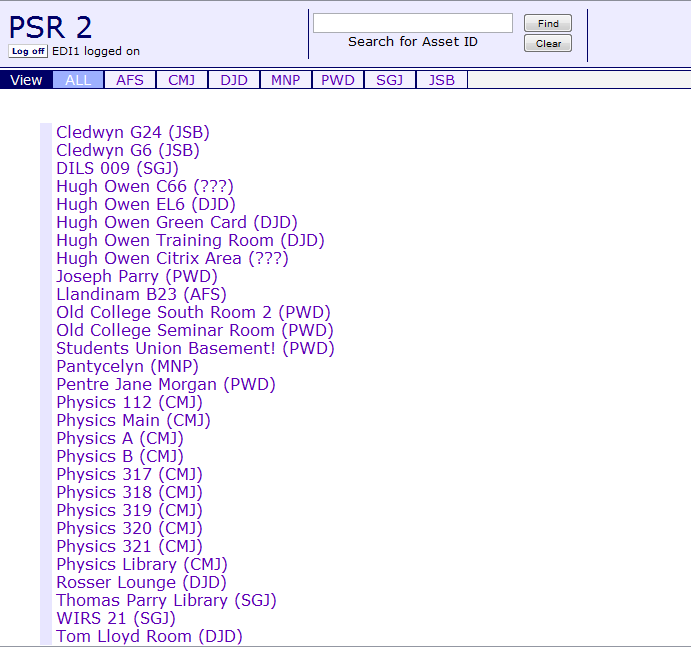
\includegraphics[scale=0.3]{./PSR2}}
\caption{Main PSR2 Page}
\label{fig:main_PSR2_page}
\end{figure}

Figure~\ref{fig:PSR2_SU_Room_layout} shows Students Union computer room layout, with the computers names and serial numbers. Room comment holds a code to unlock monitors from the security straps. It also contains the information when each computer was checked last.

It contains quite a lot of information, which is crucial to our work, and if, for some reason, the employees account will be locked we will lose access to that information, which is not held anywhere else.

\begin{figure}[H]
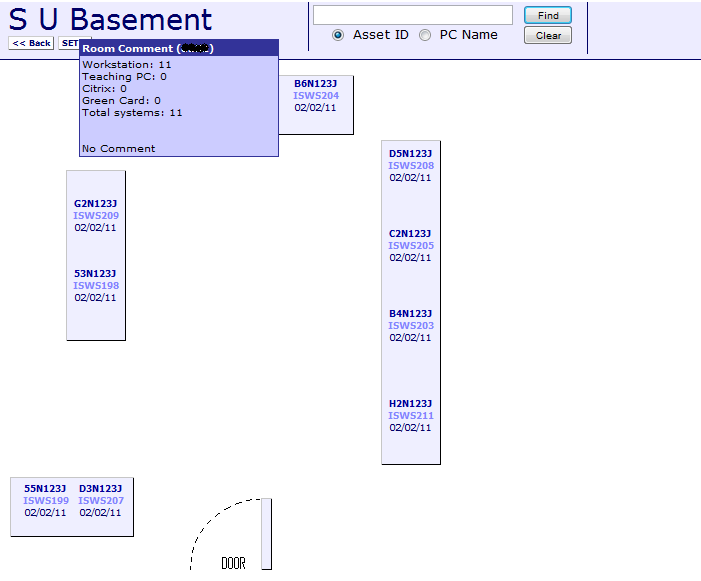
\includegraphics[scale=0.5]{./PSR2_SU_Room_layout}
\caption{PSR2 Students Union Computer Room Layout}
\label{fig:PSR2_SU_Room_layout}
\end{figure}

When I spoke to my college about the issue she explained me that this application had been written by her for herself at first and then was noticed by the team leader. He, then, asked for the other workshop members to be added on the users list. That is how thing happen sometimes: no planning, no testing, no official discussion.

\section{Summary}
As you can see there are many different programs and web interfaces to control and manage different data and services, there is no single point of control for all the systems which makes ones life a bit difficult. I understand that it may not be feasible or quite expensive to write a program that would control each and every aspect of our systems. That is one of the difficulties that I have faced in the beginning, memorising the programs names, web pages addresses and the purposes they were used for. In a few days time I did know all the essential programs names and web page addresses, but as the year passes I keep learning new ones as well.   
\chapter{What I did}
My working hours are from 8:30 until 17:00 Monday to Thursday and we have a slightly shorter day on Friday. I live just a few miles away from the University, so I get to work on foot and it usually takes me around 15 minutes to get to the office. My usual duties include computer room checks, lecturers support in teaching spaces over the phone or in person and assigned jobs completion.

My work day starts from assigned jobs review. I open Sunrise - our job management system and look through all the jobs assigned to me, then I prioritize the most important ones and plan the day accordingly. I also take a look at our list of unassigned jobs and if there are any that I can do and they look important, challenging or interesting - I assign them to myself. I would usually avoid taking difficult hardware faults with laptops since I do not officially have an appropriate qualification, but I did learn to do screen, HDD and RAM replacements. 

When I joined the IS department I had to attend compulsory training for the new staff. I was trained on how to deal with the customers in various situations, I was introduced to the IS rules, regulations and to the data protection act. I have also received the training about the user data management on reg and AStRA, IS news channels management, Voyager use - that is University's library system. I have also been shown how to use and provide support for Abercast, QMP, Qwizdom - these are the applications and tools used by the lecturers to provide better experience for the students during the lectures and seminars. I learnt to do other little things while completing the jobs and providing support to the customers, such as different customer service scenarios.

\section{Sunrise jobs}
Sunrise is the type of the jobs that I carry out on a daily basis: pick up the job, review it first, then contact the customer to arrange a visit or ask them to drop off their equipment in the workshop, fix the issue and close the job. It may sound simple, but quite often it gets unpredictable and challenging. People may forget about my visit or double book it; there also may be a situation when an urgent job appears and my team leader asks to do it first. I may go to fix one fault, but discover that the issue is completely different to the one described in the job sheet.

There are two main types of the jobs that I do, the ones that have to be done in the workshop and the ones that require a visit to the customer. The software faults would usually require physical technician presence - if the job appears in our database it means that first line fix was not available or was not enough. As for the hardware faults everything is much simpler, I just go, pick up the faulty equipment and bring it to the workshop for repair. If my work involves fixing the laptops I always send an email to the customer asking him/her to bring the laptop to the workshop whether it is a software or a hardware issue. I can then look at it more precisely in a suitable environment or ask the colleagues who are better placed than me for advice and guidance.

To give a better understanding of what I deal with I have prepared a case study. It will demonstrate the abilities and skills that I have gained during the placement. 

\subsection{Case Study}
A student has brought a laptop that would not turn on to the help desk. The fault could not be fixed at the help desk and he was offered the computer workshop services to repair his laptop. A customer expressed willingness to use our services and the job was passed to our team. I took a look at the job description and decided to take it. I believed that it would be the PSU (power supply unit) fault. There may be different issues causing the same problem: a broken power cord, faulty power supply, a broken power jack on the motherboard, wrongly seated or malfunctioning RAM, the cracks on the motherboard, CPU (Central Processing Unit) issue etc. I asked the customer to drop off the laptop in the workshop so that I could a closer look at it. 
\subsubsection{Pre check}
After receiving the laptop I checked it for the obvious damages like cracks on the casing which could indicate potential damaged of motherboard first. There was no obvious damage and it seemed to be in the good state, without marks or major scratches, kept clean and tidy. I could not smell any unusual odours from it either which could indicate that the liquid was spilled on it. After the basic pre check I questioned the customer to find out more about the issue and get a full picture. I was now ready to investigate.
\subsubsection{Investigation}
I have checked the PSU first: connected the PSU, which was provided by the customer, to the power socket to see whether it worked properly. As soon as I plugged the cable to the mains a small led light on the PSU lighted up indicating that there was an electricity flow, however, it didn't definitely mean that PSU was in the working order. The next step was to check if there was a correct voltage at the output cable. The sticker on the PSU indicated that it should provide 19 volts of DC (direct current) at the maximum of 4.74 amperes (amount of electric charge passing a point). I measured the voltage on the output by the multimeter and it reported 19 volts, the same voltage that was specified on the power supply. It was clear now that issue was not the power supply, but the laptop itself.  
\subsubsection{Computer start up}
I would like to give the reader a short overview of how the start-up process happens in the computer, from the time the power button is pressed to the time when the built in firmware passes execution to the operating system. The information is essential for the understanding of the troubleshooting technique.  

As soon as the power button is pressed the POST (Power-on self-test) process is performed by the firmware or software routines immediately after many digital electronic devices are powered on\cite{POST}. At this stage the built-in firmware checks the presence and configuration of the computer components like HDD, RAMs, CPU and the other internal components. This process may only occur if there is a power. In case there are any problems detected during that check the computer may let the user know about it by the series of signals or by display an error message on the screen. If everything works fine the firmware passes execution to the OS and the loading process continues. This is a very basic explanation for the non-technical readers. I want the reader to understand that even if there are any faulty components in PC it may still be working and you can tell that by the sound produced by the spinning plates in HDD, noise produced by the fan and by the lights in the front of the computer.
\subsubsection{Further investigation}
I have found out before that the PSU was working well and the plan was to examine the computer's behaviour. I connected the power cable and pressed the power button on the laptop to see if it starts up, but it didn't. The led light which indicates that the battery is charging was off as well. There was no "sign of life" at all: no lights on the case neither noise produced by the spinning fan or HDD, there were no error messages on the screen or signals produced by the computer to indicate an error. Clearly there was no power provided to the computer internals. I have then checked the power jack in the laptop to see if it was loose, but it looked fine, so I had no other choice than to take the laptop apart and see whether I can find any broken components inside. 
\subsubsection{Taking the laptop apart}
I have confirmed by the serial number that the laptop was not under warranty any more first. The laptops are designed to be small and portable, the components inside are pretty small, fragile and fitted close to each other. I had to be very careful when taking them apart and store all the components in a special labelled plastics boxes. I have also had to wear the grounding wrist strap to avoid electrostatic discharge which could damage sensitive components. The laptops internals usually consists of the logic board with all the components like CPU, RAMs, video card, WI-FI adapter being fitted on it. In most of the cases the HDD and CD-ROM are connected directly to the motherboard whereas a keyboard and a mouse pad are connected by the cables. 
\subsubsection{Problem discover \& fix}
When all the casing was taken away I spotted the problem straight away: it was the power jack. It seemed to be fine from the outside, but having motherboard uncovered revealed that is was dislodged from it. After soldiering the power jack back to the motherboard (figure ~\ref{fig:power jack}) and assembling the laptop back it started working straight away. To find out what the problem was I worked out the most obvious issues first then moving to the more complicated and managed to identify and fix the problem quickly and efficiently.

\begin{figure}[H]
\centering
\centerline{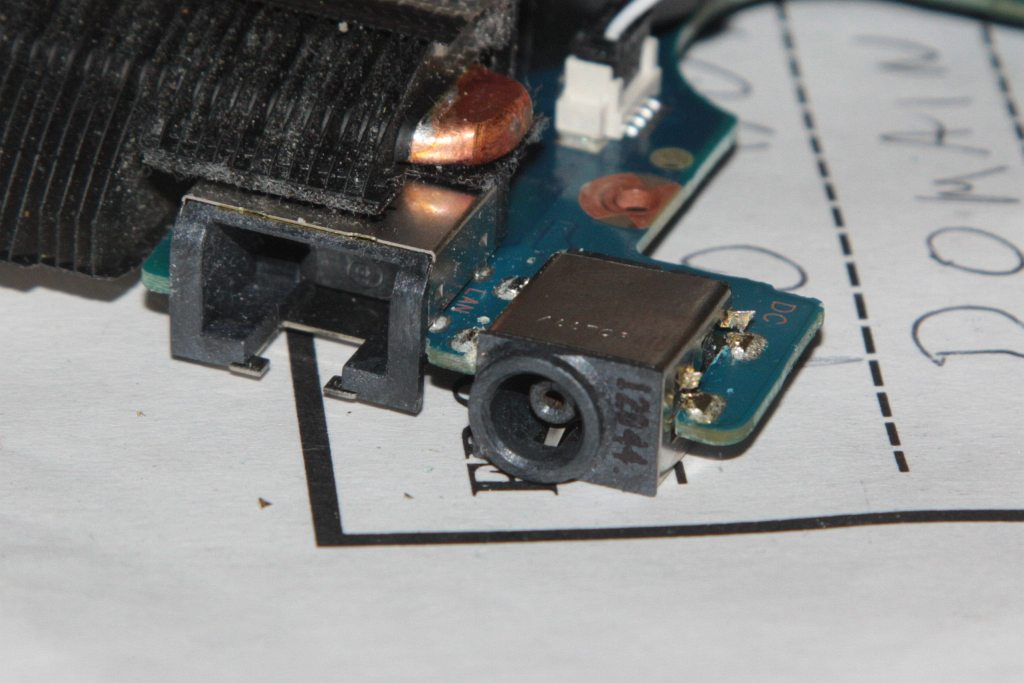
\includegraphics[scale=0.4]{./powerJack}}
\caption{Power jack on the laptop}
\label{fig:power jack}
\end{figure}

\section{Room Checks}
I have already mentioned in the section ~\ref{sec:stupid} that we perform room checks to determine any faulty ICT equipment, we tend to do it for a few times during the term time. All the permanent employees are responsible for the lecture rooms and IYs (industrial year students) take the responsibility over computer rooms. I would usually perform the room check with my colleague Daniel, he is an industrial year student as well. When performing a room check we log in to each computer in that room, this eliminates the problems with the keyboard, mouse and network (we use domain user accounts, so OS requires to fetch the data from the domain controller over the network. If user account is logged in successfully, this indicates that the network is working properly). Our job involves checking teaching equipment as well: we check whether projector performs well, the microphone and the DVD player is working and check batteries in RCs. The usual problems that we find are simple: unplugged network cables, mouse and keyboard being connected to the different computer, projector settings being changed, power cables unplugged etc. We rarely find more complex issues. During the year we have had around 5 public computers out of 500 with the hardware faults: either a broken HDD, RAM, Video Card or Motherboard. 
\section{Lecturer support}
When lecturers struggle with ICT equipment in the teaching space they can pick up a phone and it will automatically dial the workshop. It is everybody's duty in the workshop to pick up such phone calls and provide them with support. I dealt with many similar queries: usually the lecturers would ask about the way of turning on a projector, recording lectures with Panopto (lecture capture software) or they would report the microphone which does not pick up any sound. I have noticed that it isn't equipment problem in most cases but rather a user's fault, they tend not to read the notes printed for them which are located next to the equipment. Most of the problems are covered on those sheets with the solutions provided. In the first instance we try to help a user over the phone and provide them with some guidance, if a problem still persists we have to go to the lecture room to help them. When I have just started my placement I used to visit the users in most cases rather than resolving a problem over the phone. I have soon learnt how all the University's equipment is set up and managed to guide the users over the phone, saving the time for them and for myself. The biggest problem that I have faced when supporting the users over the phone was that I couldn't see what was going on, a user may describe the problem incorrectly and mislead me or miss some important piece of information. A few times I found myself solving one problem over the phone and discovering completely different issue on site. I didn't receive any relevant training so I had to develop my own techniques of troubleshooting over the phone and it took me some time to learn to ask the right questions and recognize misleading information. For example, if a user says that there is no picture on the screen I would need to work up from the most obvious reasons to the more complex. I would ask the person to check if a computer, a monitor and a projector are switched on first - the answer may seem pretty obvious, but it is not always the case. I would then ask them to switch between the video inputs (from RGB1 to RGB2) and that is the point where a problem would usually be resolved. This issue (no video output) appears if previous user used their laptop as a source of image for the projector and forgot to switch the input back to the default. I would ask a few other questions to get the full picture and would go to the lecture theatre if a problem is still not resolved to fix the issue on site.
\section{Enquiry desk}
The Enquiry desk is located in the Hugh Owen library and it provides all the users with help, such as library and IT enquiries. I am scheduled to work on the help desk twice a week for a few hours. It was completely different experience comparing to what I got used to do in the workshop. I helped the students and staff members with IT related issues, occasionally I would deal with the library questions. I would usually assist users in connecting their laptops or hand held devices to our network, activating user accounts for new students and staff, issuing new passwords, directing people in the right way, taking payments for fines, printing credit and much more. The diversity of issues to deal with is vast. When I cannot fix the problem on the help desk I make a sunrise "job" with the user details and fault description and pass it to the appropriate team. Working on the Help desk gave me a better understanding of what issues front line support staff members faced and gave me a fuller picture on how IS department operated.
  
\section{Becoming Mac Technician}
During the placement I have completed the Self-Paced Mac Technician Course. I have passed all the necessary exams and I am now a "Certified Apple Macintosh Technician". I've been provided with this amazing opportunity by the IS department and the study process proved to be tough and challenging. The average pass mark for the exam was 80\%, so there wasn't much space left to go wrong. Before starting the course I haven't known much about the Apple computers and Mac OS X, so it was an interesting course and I have learnt a lot. 

\section{Summary}
The majority of my jobs are related to hardware or software maintenance. It's a pity that I didn't have an opportunity to learn a new programming language in the organization which develops new software. However I gained experience in the computer system administration, which provides me with the opportunity to apply for a wider variety of jobs. I think this will be a valuable experience which will help me to stand out.
\chapter{Critical evaluation}
%This is the bit I really enjoy reading! This is very personal and reflective. The sort of things you might ask yourself include:
%a.       What skills did I have coming into the placement?
%b.      What were my anxieties?
%c.       What skills have I gained?
%d.      What have I learned about hierarchical organizations?
%e.      Are there any problems working in a large organization (of communication for example)
%f.        Where there issues around your environment:  how they affected work 
%and finally how you felt in the work and what you will take forward from your year Those are just a few ideas and I look forward to seeing your own

The main purpose of taking the placement for me was utilizing and evolving the skill set I had. At the end of the year I can say that the placement was of huge benefit for my career, however there wasn't particular theoretical knowledge gained which could help me with the further studies. I learnt a lot of new things: the ways of fixing diverse software and hardware issues, Windows OS configuration and domains, user account management, provision of the centrally located resources like printing and storage, user support, server side hardware and software configuration; I have also become an Apple Certified Technician, building the knowledge about the equipment produced by the company and the ways to deal with it. However, I think that the knowledge gained during the placement would not help me much with my studies, because all the skills developed are not specific to my study course. That doesn't make it useless or less beneficial, though: it was a unique opportunity to get an insight and work within the IT sector, develop the skills so essential for the environment, expand and utilize the knowledge I possessed.
\subsubsection{In IS}
When I joined the IS department I was surprised by the amount of people working there. There should be around 60 people working in the department to support the University's library and IT stuff. I think not much students and staff members realize how many people work behind the scenes to ensure that University functions. There is a team supporting networking; the one that develops new applications, other people deal with the books; I was placed within the team providing computer hardware and software support. I have had some previous experience in supporting MS Windows OS for the friends and the family as well as having hardware knowledge since I have built a few computers from the components before. I think I was placed within this team because I have expressed a deep interest in the computer hardware on the interview day.

\subsubsection{At work}
During the first few weeks I was afraid that my knowledge may not be sufficient enough to perform well at work, but as the time passed I got the ropes. I have noticed that there are similarities in the software faults like MS Outlook, EndNote, VPN connections, browser problems and, of course, Windows OS itself. Nobody expected me learn everything at once and I was taught gradually over the year. I have gained a lot of knowledge during the placement. In the workshop I learnt the technical stuff like taking laptops and PCs apart, improved my soldiering skills, learnt some different techniques of trouble shooting hardware and software issues. I enjoyed working with hardware because it is particularly interesting to me. The people I was working with were very helpful and could provide me with advice on any question that I had. My team leader was good as well providing me with support when I needed it, however he could be quite demanding, asking me to do another jobs right in the middle of the work I was doing or just before the visit to the customer that was arranged. I suppose it will happen quite often in the industry I intend to work in, because it is certainly a fast-paced one, so multi-tasking is a key. It took me around three months to understand properly how the organization and systems functioned to preform the jobs on my own without asking for help. By the end of the day it was about knowing some small bits and pieces of information to perform well at work. I was on call once and a gentleman asked me why his phone didn't work. It was the first time then that I had to deal with such query and I had no idea of who was responsible for configuring the phones in IS. I took the contact details of the customer and returned to the workshop, where I was told that phones were managed by Systems team and I should speak to them. I could, then, redirect the customer to them.

\subsubsection{Interacting with people}
It was about interacting with people from the other teams as well, if I needed working network point at some location, I had to speak with somebody from the Networking team and they would do it for me. During the first weeks of my placement when I needed assistance from the other teams I would be told to "go and speak to those people, but no one would explain me who to speak to in particular or what should I ask for? I had to find it out myself and I did look silly asking wrong questions in the beginning, indeed. But that is the way you learn to do things.

\subsubsection{Useful ideas}
While working in IS I saw how IT provision is provided in big organization, I could learn from the inside what applications and services are used and how they are configured. End user just sees front end which is provided for them, but there are loads of things going behind the scenes as well. I gathered loads of ideas and clever solutions to the common problems, I would like to mention some of them. Computers across the campuses are configured in such a way that anybody who have user account can logon on to them. This is achieved by all of them being members of Windows domain, which allows easier management and maintenance of large number of computers running under Windows OS. Central printing is another nice technique which I rely liked, idea is to have one virtual printer where user sends print job and then can print it on any printer connected to the server. Windows imaging (with help of Symantec Ghost Cast) which allows deployment of Windows OS on large amounts of computers in a short time. Another cool tool that I used is MS Windows Sysprep, it allows to prepare Windows image with all required programs for the later deployment. I even created my own Windows 7 build image for the home use, were I have all programs that I like already incorporated in to the image, so that after installation I don't need to spend hours installing drivers and other applications. Use of VLANs another cool technique which I made a not of for the future use, it allows for devices in different physical locations, not going back to the same router, be on the same network. This way making network more secure or providing people in different physical locations with the access to shared resources. Windows Remote Assistance which is used to see users screen and control mouse with keyboard, this way being able to resolve some minor issues without leaving the office.

Even now when it is time to leave I feel that there is still loads of things which I could learn. At the end my IY I was offered part-time position for a year as a casual customer services assistant which I accepted. 

\bibliographystyle{ieeetr}
\bibliography{bibl}

\end{document}